\documentclass{article}
\usepackage[utf8]{inputenc}

\title{Analysis_1_V1.0}
\author{thi.schwaller444 }
\date{December 2019}
\usepackage{graphicx}
\usepackage{mathtools}
\usepackage[a4paper,width=150mm,top=25mm,bottom=25mm]{geometry}
\pagestyle{myheadings}
\markright{Thierry Schwaller / https://github.com/tschwall/Zusammenfassungen}
\usepackage{multicol}
\begin{document}
\section{Kapitel 1: Reele Zahlen}
	\subsection{Summen / Reihen}
	\begin{itemize}
		\item sup(Menge) = "beste" obere Schranke
		\item inf(Menge) = "beste" untere Schranke
		\item sup und inf sind maximum und minimum wenn sie im Zahlenbereich enthalten sind
	\end{itemize}
	\subsection{Intervall}
	Ein Intervall ist ein Ausschnitt aus dem Zahlenstrahl
	\begin{equation}
		\textrm{Abgeschlossenes Intervall: } [a;b] = \left\{ x \in R \mid a \le x \le b \right\}
	\end{equation}
	\begin{equation}
	\textrm{Offenes Intervall: } (a;b) = \left\{ x \in R \mid a < x < b \right\}
	\end{equation}
		\subsection{Binominalzahlen / Binomischer Satz S.12}
	Binominalzahl:
	\begin{equation}
		c(k,n) = \binom{n}{k} = \textrm{Anzahl Möglichkeiten} = \frac{n(n-1)(n-2) \dots (n-k+1)}{k!} = \frac{n!}{k!(n - k)!}
	\end{equation}
	\begin{multicols}{2}
		\textbf{Binomischer Satz:}
	\begin{equation}
		(a+b) ^n = \sum_{k = 0}^{n} \binom{n}{k} a^{n-k} * b^k
	\end{equation}
	\columnbreak
	\begin{center}
	    	\begin{equation}
	    \binom{n}{0} = 1
	\end{equation}
	\end{center}
	\end{multicols}
    \subsection{Beweisen S.5}
	\subsubsection{Vollständige Induktion}
	\begin{multicols}{2}
	\begin{center}
	    \textbf{Verankerung} \\
		Beweisen für erstes n(meistens n = 1)
	\end{center}
		\columnbreak
		\begin{center}
		    \textbf{Vererbung} \\
		    Annahme: Formel korrekt für n \\
		    Schritt: Beweisen das Formel korrekt für n + 1
		\end{center}
	\end{multicols}
	\subsection{Ungleichungen S.30}
	\begin{multicols}{2}
	\begin{center}
	\textbf{Bernouli-Ungleichung}
	    	\begin{equation}
		    (1 + a) ^ n > 1 + n * a
	    \end{equation}
	\end{center}
	\columnbreak
	\begin{center}
	\textbf{Binomische-Ungleichung}
	    \begin{equation}
		|a*b| \leq \frac{1}{2}(a^2 + b^2)
	    \end{equation}
	\end{center}
	\end{multicols}
	\textbf{Mittelwerte Ungleichung}
	\begin{equation}
		\textrm{Harm. Mittel (HM) } \leq \textrm{Geom. Mittel (GM) } \leq \textrm{Arit. Mittel (AM) }
	\end{equation}
	\newpage
		\section{Kapitel 2: Funktionen}
		\begin{multicols}{2}
		\subsection{Begriffsdefinition S.59}
	\begin{itemize}
		\item f ungerade $\rightarrow$ f(-x) = -f(x) (Punktsymmetrisch an (0,0))
		\item f ungerade $\rightarrow$ f hat nur ungerade Potenzen
		\item f gerade f(-x) = f(x) (Graph symmetrisch zur y-Achse)
		\item Umkehrbarkeit $f^{-1}$ "Von Wert y $\rightarrow$ x" (Output zu Input) 
		\subitem y = f(x) $\rightarrow$ $x = f^{-1}(y)$
		\item Restriktion Teil einer Funktion 
		\item Monotonie ((streng) monoton steigend,(streng) monoton fallend)
	\end{itemize}
	\columnbreak
	\subsection{Elementare Transformation}
	Immer zuerst Strecken und dann verschieben. Schrittweise Vorgehen
	\begin{itemize}
	    \item \textbf{x: Verschiebung} (x-b) anstatt x $\rightarrow$ f(x-b) (b in x-Richtung)
	    \item \textbf{x: Streckung} a * x statt x $\rightarrow$ f(a*x) (Streckfaktor ist $\frac{1}{a}$)
	    \item \textbf{y: Verschiebung} y = f(x) + B (B in y-Richtung)
	    \item \textbf{y: Streckung} y = f(x) * A
	\end{itemize}
		\end{multicols}
	\subsection{Horner-Zerlegung S.967}
	Wird für die Zerlegung von polynomischen Funktionen gebraucht.(P.B.Z)
	\begin{equation}
		f(x) = (x - x_1) * (b_{n-1}x^{n-1} + b_{n-2}x{n-2} + \dots + b_2x^2 + b_1x + b_0) 
	\end{equation}
	Spezialfall f($x_1$) = 0 $\rightarrow$ Schema liefert Faktorzerlegung 
	\begin{center}
	    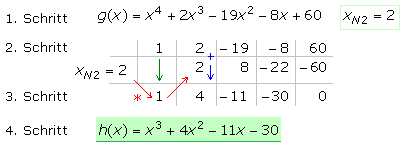
\includegraphics[width=0.35\textwidth]{Horner.png}
	\end{center}
	\subsection{Gebrochene Funktionen S.15}
	\begin{equation}
			\frac{\textrm{Polynom im Zähler}}{\textrm{Polynom im Nenner}}
	\end{equation}
	Wichtig: Nennernullstellen wegnehmen aus Definitionsbereich
	\subsection{Partialbruch Zerlegung P.B.Z S.15}
	\begin{enumerate}
		\item Echt gebrochen? Nennergrad $>$ Zählergrad 
		\item Nenner faktorisieren ! Geht immer mindestens bis Grad 2
		\subitem Zerlegungsansatz $\frac{\textrm{Zähler 1}}{\textrm{Faktor 1}} + \frac{\textrm{Zähler 2}}{\textrm{Faktor 2}} + \dots + \frac{\textrm{Zähler n}}{\textrm{Faktor n}}$
		\subitem Berechnen der Zähler 1 bis n (Einsetzen, Koeffizientenvergleich)
	\end{enumerate}
	\subsection{Hyperbolische Funktionen Sinh / Cosh S.89 Area S.94}
	\begin{multicols}{2}
	\begin{center}
	\begin{equation*}
	    cosh(x) = \frac{1}{2}(e^x+e^{-x})
	\end{equation*}
	\end{center}
	\columnbreak
	\begin{center}
	\begin{equation*}
	    sinh(x) = \frac{1}{2}(e^x+e^{-x})
	\end{equation*}
	\end{center}
	\end{multicols}
	
	\newpage
		\section{Kapitel 3: Folgen}
	\subsection{Allgemein}
	Folgen = Funktionen f(N) $\rightarrow$ R ; f(1) = $f_1$ \\
	Geometrische Folge $\rightarrow a_1q^{n-1}$ $(q \in R)$ \\
	Beschränkt: $W_f \in$ endliches Intervall \\ \\
	Monotonie: \\
	streng monoton sinkend $\rightarrow$ $f_{n+1} < f_n (n \in N)$ $f_{n+1} - f_n < 0; \frac{f_{n+1}}{f_n} < 1$ $(f_n > 0)$ \\
	streng monoton steigend $\rightarrow$ $f_n < f_{n+1}$ $(n \in N)$
	\subsubsection{Begriffe S.470}
	\begin{itemize}
		\item Konvergent $\rightarrow$ Die Werte nähern sich immer mehr einem Wert in R an 
		\item Bestimmte Divergenz $\rightarrow$ Die Werte nähern sich entweder -$\infty$ oder $\infty$ an
		\item Unbestimmte Divergenz $\rightarrow$ Die Werte nähern sich keinem bestimmten Wert an 
		\item Einschwingen $\rightarrow$ $ a_n$ alterniert (wechselt zwischen + und - bei jedem Schritt) und $\lim\limits_{n \rightarrow \infty a_n}$ = 0
		\item Partialsumme $\rightarrow s_n = \sum_{i = 1}^{n} (a_i)$ 
	\end{itemize}
	\subsection{Rekursion}
	Eine rekursive Fomel ist eine Formel in welche das nächste Element durch die vorhergehenden Werte ausgedrückt wird (Fibonacci-Folge).
	\begin{equation}
		f_{n+1} = \textrm{Formel aus } f_n;f_{n-1}; \dots ; f_1 (n \in N, \textrm{Initialwert } f_1 \textrm{ mind. benötigt})
	\end{equation}
	\textbf{Satz von Bolzano:} Jede monoton beschränkte Folge konvergiert. \\
	\textbf{Konvergenz: } $n+1 = n$
	\subsection{Eulerische Zahl / Exponentialfunktionen S.478}
	\begin{equation}
	    e^x \leq \frac{1}{1-x}
	\end{equation}
		\begin{equation}
	    e^{\ln(x)} = x
	\end{equation}
	\begin{equation}
	    e =\lim\limits_{n \rightarrow \infty} (1 + \frac{1}{n})^n \rightarrow \textrm{Konvergiert!}
	\end{equation}
	\begin{equation}
	    e^x =\lim\limits_{n \rightarrow \infty} (1 + \frac{x}{n})^n \rightarrow \textrm{Konvergiert!}
	\end{equation}
	\begin{equation*}
	    e^x \geq 1 + x
	\end{equation*}
	Dies ist eine monoton steigende Funktion ohne Sprünge.
	\newpage
		\section{Grenzwerte f}
		Funktion $\rightarrow$ S.54
		Reihen $\rightarrow$ S. 472
	\subsection{Grenzwerte}
	\begin{itemize}
		\item Spez. Gesetze mit + und - $\infty$
		\item Konvergenz kann mit normalen Operationen berechnet werden / Grenzwerte verrechnen sich wie Zahlen
	\end{itemize}
	\subsection{Grenzwert Berechnungen}
	Mit einsetzen der Grenzwerte von verschiedenen "einfacheren" Termen kann ein "komplizierterer" berechnet werden. \\ \\
	Option 1: Erweitern $\rightarrow$ Division höchster Potenz \\
	Option 2: Erweitern $\rightarrow$ Gegenterm (+ und - tauschen) \\
	Option 3: Einschliessung $a_n \leq c_n \leq b_n$ \\
	Option 4: Bernoulli - Hopital Gleichung: (nur wenn $\frac{0}{0}, \frac{\infty}{\infty}, 0 * \infty, \infty - \infty, 0^0,\infty^0, 1^\infty$) \\
	Wenn  $\frac{0}{0}, \frac{\infty}{\infty}$: 
    \begin{center}
    Bronstein Seite 57
    \end{center}
	\subsection{Asymptoten / Polstellen}
	\begin{itemize}
	    \item \textbf{Polstellen} $\rightarrow$ Unbestimmte Punkte in einer Funktion
	    \item \textbf{Asymptoten} $\rightarrow$ Nenner durch Zähler dividieren (ganzrat. F (=Asymtote) + echt gebrochenen F)
	\end{itemize}
	\begin{center}
	    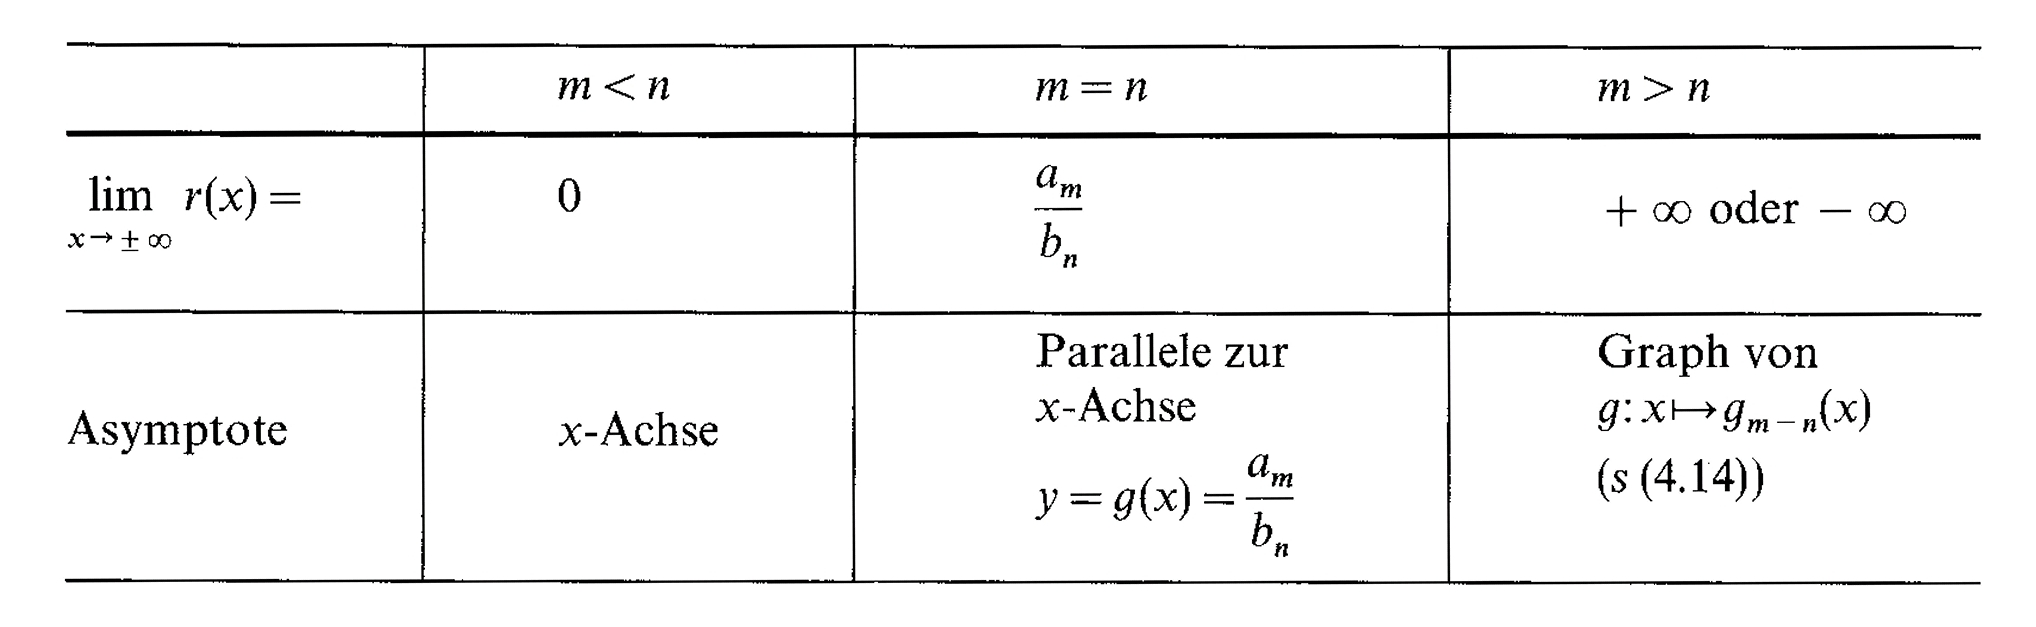
\includegraphics[width=0.5\textwidth]{Asymptote.jpg}
	\end{center}
	\subsection{Übertragungsprinzip}
	\subsection{Stetigkeit}
	Eine Stetige-Funktion ist eine Funktion welche mit einem Strich ohne absetzen gezeichnet werden kann. Es gibt drei Arten von unstetigen Funktionen: 
	\begin{itemize}
	    \item \textbf{Hebbare Funktionen} Definitionslücken (zum Beispiel x = 1 ist unbestimmt)
	    \begin{equation}
	        \frac{x^2 + 1}{x - 1}
	    \end{equation}
	    \item \textbf{Sprung / 1. Art} $g^+$ und $g^-$ existieren sind aber ungleich. (Sprung zwischen zwei aufeinander folgenden Werten)
	    \item \textbf{2. Art} Oszilattion / $g^+$ oder $g^-$ existieren in $x_0$ nicht
	\end{itemize}
\end{document}
